% 广义曲线坐标系拉普拉斯算子证明

\section{尝试证明}%
我们电动力学书上是直接给出梯度散度旋度拉普拉斯算符的,我对此一直很困惑

\begin{definition}[梯度]
	\begin{equation}
		\grad = \sum_i \frac{1}{\textcolor{red}{h_i}} \red{\pdv{x_i}} \vu{x}_i
		\label{eq:梯度}
	\end{equation}
\end{definition}

\begin{definition}[散度]
	\begin{equation}
		\label{eq:div}
		\div \vb{y}  = \frac{1}{\prod_i h_i} \sum_i \left[
			\pdv{x_i}( h'_i \red{y_i})
			\right]
		\qc
		h'_{i} = \prod_{j \neq i}  h_j
	\end{equation}
\end{definition}

我发现:\\
只要令 Eq.~\eqref{eq:div} 中 $\vb{y}$ 等于 $\grad$ \\
即:令$y_i=\frac{1}{\textcolor{red}{h_i}} \red{\pdv{x_i}} $ 塞进 Eq.~\eqref{eq:div}
\begin{definition}[拉普拉斯算子]

	\begin{equation}
		\div \grad \equiv \laplacian = \frac{1}{\prod_i h_i}
		\sum_i
		\left[
			\pdv{x_i}( \frac{h'_i}{\red{h_i}} \red{\pdv{x_i}})
			\right]
		\qc
		H_i = \frac{\prod_{j \neq i} h_j}{ h_i } =\frac{h'_i}{ h_i }
    \label{eq:广义曲线坐标系拉普拉斯算子}
	\end{equation}
\end{definition}


\begin{definition}[旋度]
	\begin{equation}
		\curl \vb{y}  = \frac{1}{\prod_i h_i}
		\begin{vmatrix}
			\ldots & h_i  \vu{x}_i & \ldots \\
			\ldots & \pdv{x_i}     & \ldots \\
			\ldots & h_i y_i       & \ldots
		\end{vmatrix}
	\end{equation}
\end{definition}
先证明梯度,其他看起来大同小异。
直接列式子要写一大堆,用线性代数矩阵乘法来做要简洁些(满足结合律)。
\section{开始证明}%
\subsection{铺垫}%
\subsubsection{旋转矩阵}%
% 基矢变换
\begin{figure}[h]
	\centering
	\includesvg[width=0.3\linewidth]{figures/坐标系变换}
	\caption{直角坐标基矢变换为极坐标基矢}%
	% \label{fig:fig/坐标系变换}
\end{figure}

\begin{equation}
	\begin{aligned}
		% \label{eq:坐标变换方程}
		\vu{r}     & = \cos\phi \vu{i} + \sin\phi \vu{j}                                    \\
		\vu*{\phi} & = \cos(\phi+ \frac{\pi}{2}) \vu{i} + \sin(\phi + \frac{\pi}{2} )\vu{j}
	\end{aligned}
\end{equation}




写成矩阵形式

\begin{equation}
	% \label{Eq:矩阵形式的坐标变换}
	\mqty[ \vu{r} \\ \vu*{\phi}  ] =
	\mqty[
		\cos\phi & \sin\phi \\
		-\sin\phi &\cos\phi \\
	]
	\mqty[ \vu{i} \\ \vu{j} ]
\end{equation}

\begin{definition}[旋转矩阵\(\RHat\)]
	\begin{equation}
		\RHat =
		\mqty[
			\cos\phi & \sin\phi \\
			-\sin\phi &\cos\phi \\
		]
		\label{eq:旋转矩阵}
	\end{equation}
\end{definition}

\begin{remark}
	极坐标的旋转矩阵 好写,就是看图转下,\(\phi\) 多加 90度; 柱坐标也好写,在极坐标基础上多加一维;球坐标的旋转矩阵,就是在柱坐标基础上再转下,在柱坐标旋转矩阵基础上再乘一个矩阵
\end{remark}

通过观察法凑出基矢变换矩阵(对于球坐标也就是转两次的“旋转矩阵”)可以这样写:
\begin{equation}
    \label{eq:基矢变换矩阵}
  \begin{aligned}
    \RHat &=
  \mqty[
  \frac{1}{h_1} \pdv{x}{r} &
  \frac{1}{h_1} \pdv{y}{r} &
  \frac{1}{h_1} \pdv{z}{r} \\
  \frac{1}{h_2} \pdv{x}{\theta} &
  \frac{1}{h_2} \pdv{y}{\theta} &
  \frac{1}{h_2} \pdv{z}{\theta} \\
  \frac{1}{h_3} \pdv{x}{\phi} &
  \frac{1}{h_3} \pdv{y}{\phi} &
  \frac{1}{h_3} \pdv{z}{\phi} \\] \\
        &=
        \mqty[
  \frac{1}{h_1}  &
  0  &
  0  \\
  0  &
  \frac{1}{h_2}  &
  0  \\
  0  &
  0  &
  \frac{1}{h_3}  \\
        ]
\mqty[
  \pdv{x}{r} &
  \pdv{y}{r} &
  \pdv{z}{r} \\
  \pdv{x}{\theta} &
  \pdv{y}{\theta} &
  \pdv{z}{\theta} \\
  \pdv{x}{\phi} &
  \pdv{y}{\phi} &
  \pdv{z}{\phi} \\] \\
                & = 
        \mqty[
  \frac{1}{h_1}  &
  0  &
  0  \\
  0  &
  \frac{1}{h_2}  &
  0  \\
  0  &
  0  &
  \frac{1}{h_3}  \\
        ]
        \JJ \tp
  \end{aligned}
\end{equation}


\vspace{1cm}
\subsubsection{雅可比矩阵}%
\begin{definition}[雅可比矩阵]
	\begin{equation}
		\label{eq:雅可比矩阵}
		\begin{aligned}
			\JJ             & =
			\left(
			\left(\pdv{\vb{x}}\right) \left(\vb{y}\right)\tp
			\right)\tp
			=
			\left(
			\begin{pmatrix}
					\pdv{r}      \\
					\pdv{\theta} \\
					\pdv{\phi}
				\end{pmatrix}
			\begin{pmatrix}
					x & y & z
				\end{pmatrix}
			\right)\tp                                                  \\
			                & =
			\pdv{(x,y,z)}{(r,\theta,\phi)}
			=
			\mqty[
			\pdv{x}{r}      & \pdv{x}{\theta}      & \pdv{x}{\phi}      \\
			\pdv{y}{r}      & \pdv{y}{\theta}      & \pdv{y}{\phi}      \\
			\pdv{z}{r}      & \pdv{z}{\theta}      & \pdv{z}{\phi}
			]
			=
			\mqty[
			\pdv{\vb{r}}{r} & \pdv{\vb{r}}{\theta} & \pdv{\vb{r}}{\phi}
			]
		\end{aligned}
	\end{equation}
\end{definition}

\vspace{1cm}
\subsubsection{拉梅系数}
\begin{equation}
  \label{eq:拉梅系数}
	h_i=\norm{\pdv{\vb{\vb{y}}}{x_i}} \qq{或写成}
	h_i=\norm{\pdv{\vb{\vb{r}}}{q_i}}
\end{equation}
\marginnote{看起来对雅可比矩阵的一列取模就是拉梅系数的值了?}
如表\ref{tab:lamei}所示。
\begin{table}[htpb]
	\centering
	\caption{拉梅系数.}
	\label{tab:lamei}
	\begin{tabular}{c|ccc}
		\toprule
		$(q_1,q_2,q_3)$ & 直角$(x,y,z) \tp$ & 柱 $(\rho, \phi, z) \tp$ & 球 $(r, \theta, \phi) \tp$ \\
		\midrule
		$h_1$           & $1$               & $1$                      & $1$                        \\
		$h_2$           & $1$               & $\rho$                   & $r$                        \\
		$h_3$           & $1$               & $1$                      & $r\sin\theta$              \\
		\bottomrule
	\end{tabular}
\end{table}
\subsection{证明的关键:旋转矩阵乘雅可比行列式}%
利用链式法则和式~\eqref{eq:雅可比矩阵} 可得
\begin{equation}
	\label{eq:链式法则}
	\mqty[
		\pdv{u}{r} \\ \pdv{u}{\phi}
		\\ \pdv{u}{\theta}
	]
	=
	\mqty[
		\pdv{x}{r} & \pdv{x}{\phi} & \pdv{x}{\theta} \\
		\pdv{y}{r} & \pdv{y}{\phi} & \pdv{y}{\theta} \\
		\pdv{z}{r} & \pdv{z}{\phi} & \pdv{z}{\theta} \\
	] \tp
	\mqty[
		\pdv{u}{x} \\ \pdv{u}{y}
		\\ \pdv{u}{z}
	]
	= \JJ \tp
	\mqty[
		\pdv{u}{x} \\ \pdv{u}{y}
		\\ \pdv{u}{z}
	]  \\
\end{equation}
\begin{equation*}
	\mqty[
		\pdv{u}{x} \\ \pdv{u}{y}
		\\ \pdv{u}{z}
	]
	=
	\mqty[
		\pdv{r}{x} & \pdv{\phi}{x} & \pdv{\theta}{x} \\
		\pdv{r}{y} & \pdv{\phi}{y} & \pdv{\theta}{y} \\
		\pdv{r}{z} & \pdv{\phi}{z} & \pdv{\theta}{z} \\
	]
	\mqty[
		\pdv{u}{r} \\ \pdv{u}{\phi}
		\\ \pdv{u}{\theta}
	]
	= (\JJ  \tp)^{-1}
	\mqty[
		\pdv{u}{r} \\ \pdv{u}{\phi}
		\\ \pdv{u}{\theta}
	]
\end{equation*}
\begin{equation*}
	\mqty[
		\pdv{u}{x} \\ \pdv{u}{y}
		\\ \pdv{u}{z}
	] \tp
	=
	\mqty[
		\pdv{u}{r} \\ \pdv{u}{\phi}
		\\ \pdv{u}{\theta}
	] \tp
	\mqty[
		\pdv{r}{x} & \pdv{\phi}{x} & \pdv{\theta}{x} \\
		\pdv{r}{y} & \pdv{\phi}{y} & \pdv{\theta}{y} \\
		\pdv{r}{z} & \pdv{\phi}{z} & \pdv{\theta}{z} \\
	] \tp
	= ((\JJ  \tp)^{-1})\tp
	\mqty[
		\pdv{u}{r} \\ \pdv{u}{\phi}
		\\ \pdv{u}{\theta}
	]
	= \JJ^{-1}
	\mqty[
		\pdv{u}{r} \\ \pdv{u}{\phi}
		\\ \pdv{u}{\theta}
	]
\end{equation*}
直角坐标的梯度可以这样写:
\begin{equation}
	\label{eq:直角坐标梯度}
	\begin{aligned}
		\grad u    & =
		\mqty[
		\pdv{u}{x} & \pdv{u}{y}
		           & \pdv{u}{y}
		]
		\mqty[
		\vu{i}                  \\
		\vu{j}                  \\
		\vu{k}                  \\
		]                       \\
	\end{aligned}
\end{equation}
把式~\eqref{eq:旋转矩阵}和式~\eqref{eq:链式法则} 带入式~\eqref{eq:直角坐标梯度},并把式~\eqref{eq:梯度}写成矩阵形式:
\begin{equation}
	\begin{aligned}
		\grad u       & =
		\mqty[
		\pdv{u}{r}    & \pdv{u}{\phi}
		              & \pdv{u}{\theta}
		]
		\red{\JJ^{-1} \RHat \tp
		}\mqty[
		\vu{r}                                          \\
		\vu{\phi}                                       \\
		\vu{\theta}                                     \\
		]                                               \\
		              & =
		\mqty[
		\pdv{u}{r}    & \pdv{u}{\phi}
		              & \pdv{u}{\theta}
		]
		\red{\mqty[
		\frac{1}{h_1} & 0               & 0             \\
		0             & \frac{1}{h_2}   & 0             \\
		0             & 0               & \frac{1}{h_3}
			]}
		\mqty[
		\vu{r}                                          \\
		\vu{\phi}                                       \\
		\vu{\theta}                                     \\
		]                                               \\
	\end{aligned}
\end{equation}
\marginnote{我猜想红色的式子是普遍相等的}

\begin{equation*}
	\JJ^{-1} \RHat \tp
	=
	\mqty[
		\frac{1}{h_1} &0&0 \\
		0&\frac{1}{h_2}&0 \\
		0&0&\frac{1}{h_3}
	]
\end{equation*}

\begin{equation*}
	(\JJ^{-1} \RHat \tp)^{-1}
	=
	\RHat \JJ
	=
	\mqty[
		h_1 &0&0 \\
		0&h_2&0 \\
		0&0& h_3
	]
\end{equation*}
将式~\eqref{eq:基矢变换矩阵} 带入:
\begin{equation*}
  \begin{aligned}
    \RHat \JJ &= 
        \mqty[
  \frac{1}{h_1}  &
  0  &
  0  \\
  0  &
  \frac{1}{h_2}  &
  0  \\
  0  &
  0  &
  \frac{1}{h_3}  \\
        ]
\mqty[
  \pdv{x}{r} &
  \pdv{y}{r} &
  \pdv{z}{r} \\
  \pdv{x}{\theta} &
  \pdv{y}{\theta} &
  \pdv{z}{\theta} \\
  \pdv{x}{\phi} &
  \pdv{y}{\phi} &
  \pdv{z}{\phi} \\]
			\mqty[
			\pdv{x}{r}      & \pdv{x}{\theta}      & \pdv{x}{\phi}      \\
			\pdv{y}{r}      & \pdv{y}{\theta}      & \pdv{y}{\phi}      \\
			\pdv{z}{r}      & \pdv{z}{\theta}      & \pdv{z}{\phi}
			] \\
                      &=
        \mqty[
  \frac{1}{h_1}  &
  0  &
  0  \\
  0  &
  \frac{1}{h_2}  &
  0  \\
  0  &
  0  &
  \frac{1}{h_3}  \\
        ] 
        \JJ \tp \JJ
  \end{aligned}
\end{equation*}

也就是证明:
\begin{equation}
  \label{eq:拉梅系数平方}
        \JJ \tp \JJ
        =
        \mqty[
        h_1^2 & 0 & 0 \\
        0 & h_2^2 & 0 \\
        0 & 0 & h_3^2 \\
        ]
\end{equation}
由拉梅系数定义式~\eqref{eq:拉梅系数} 知,只需要证明雅可比矩阵正交

% \inputminted[linenos,numbersep=5pt,frame=lines,framesep=2mm]{wolfram}{./j.mma}
\code{wolfram}{./j.mma}
用 Mathematica 验证发现对于极坐标,柱坐标,球坐标,雅可比矩阵都满足式~\eqref{eq:拉梅系数平方} 。
% \(\RHat \JJ =\text{\mintinline{matlab}{diag([h1,h2,h3])}}\)
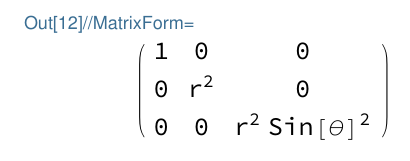
\includegraphics[width=0.5\textwidth]{figures/2021-10-13T133210+0800.png} 


\subsection{没证明出来的地方}%
\begin{itemize}
  \item 如果给出任意变换,如何写出基矢变换矩阵~\eqref{eq:基矢变换矩阵} 
  \item 雅可比矩阵正交
\end{itemize}


%%% vim: set ts=2 sts=2 sw=2 isk+=\: et cc=+1 formatoptions+=mM:
